% \subsection{Mục tiêu đề tài}

% Nhằm vượt qua những thách thức cố hữu và khai thác tối đa tiềm năng trong từng giai đoạn của hành trình khách hàng, nhóm nghiên cứu đã phát triển một ứng dụng tích hợp, được thiết kế chuyên biệt để nâng tầm trải nghiệm cho khách hàng, nhân viên và quản lý nhà hàng. Ứng dụng này tập trung vào việc cải thiện các điểm chạm then chốt trong hành trình khách hàng, tạo ra một quy trình liền mạch và hiệu quả hơn:
% \begin{enumerate}
%     \item Giai đoạn Cân nhắc (Consideration):     Ứng dụng cho phép khách hàng dễ dàng truy cập thực đơn trực tuyến chi tiết, hình ảnh chất lượng cao về món ăn và không gian nhà hàng, cũng như các đánh giá từ những khách hàng khác. Chức năng so sánh giá cả và tùy chọn tùy chỉnh món ăn giúp khách hàng đưa ra quyết định sáng suốt..
%     \item Giai đoạn Trải nghiệm (Experience): Ứng dụng cung cấp các tính năng hỗ trợ trong quá trình trải nghiệm tại nhà hàng, bao gồm một vài tính năng cơ bản như:
%         \begin{itemize}
%             \item \textit{Gọi món qua ứng dụng:} Khách hàng có thể dễ dàng xem thực đơn và gọi món trên điện thoại thông minh của mình.
%             \item \textit{Gửi yêu cầu trực tiếp đến nhân viên phục vụ:} Giúp tăng cường tương tác và giải quyết các vấn đề nhanh chóng.
%             \item \textit{Thu thập phản hồi thời gian thực:} Cho phép nhà hàng đánh giá và cải thiện chất lượng dịch vụ ngay lập tức.
%         \end{itemize}
%     \item Giai đoạn Thanh toán (Payment): Ứng dụng tích hợp nhiều phương thức thanh toán điện tử (thẻ tín dụng, ví điện tử), cho phép khách hàng thanh toán nhanh chóng và an toàn. Hóa đơn điện tử được tạo tự động và gửi trực tiếp đến khách hàng.
%     \item Giai đoạn Hậu trải nghiệm (Post-Experience): Ứng dụng hỗ trợ gửi email cảm ơn tự động, khuyến khích khách hàng để lại đánh giá và tham gia chương trình khách hàng thân thiết. Dữ liệu về lịch sử mua hàng và sở thích của khách hàng được sử dụng để cá nhân hóa các ưu đãi và khuyến mãi, tăng khả năng quay lại của khách hàng.

% \end{enumerate}

% \begin{figure}[H]
%     \centering
%     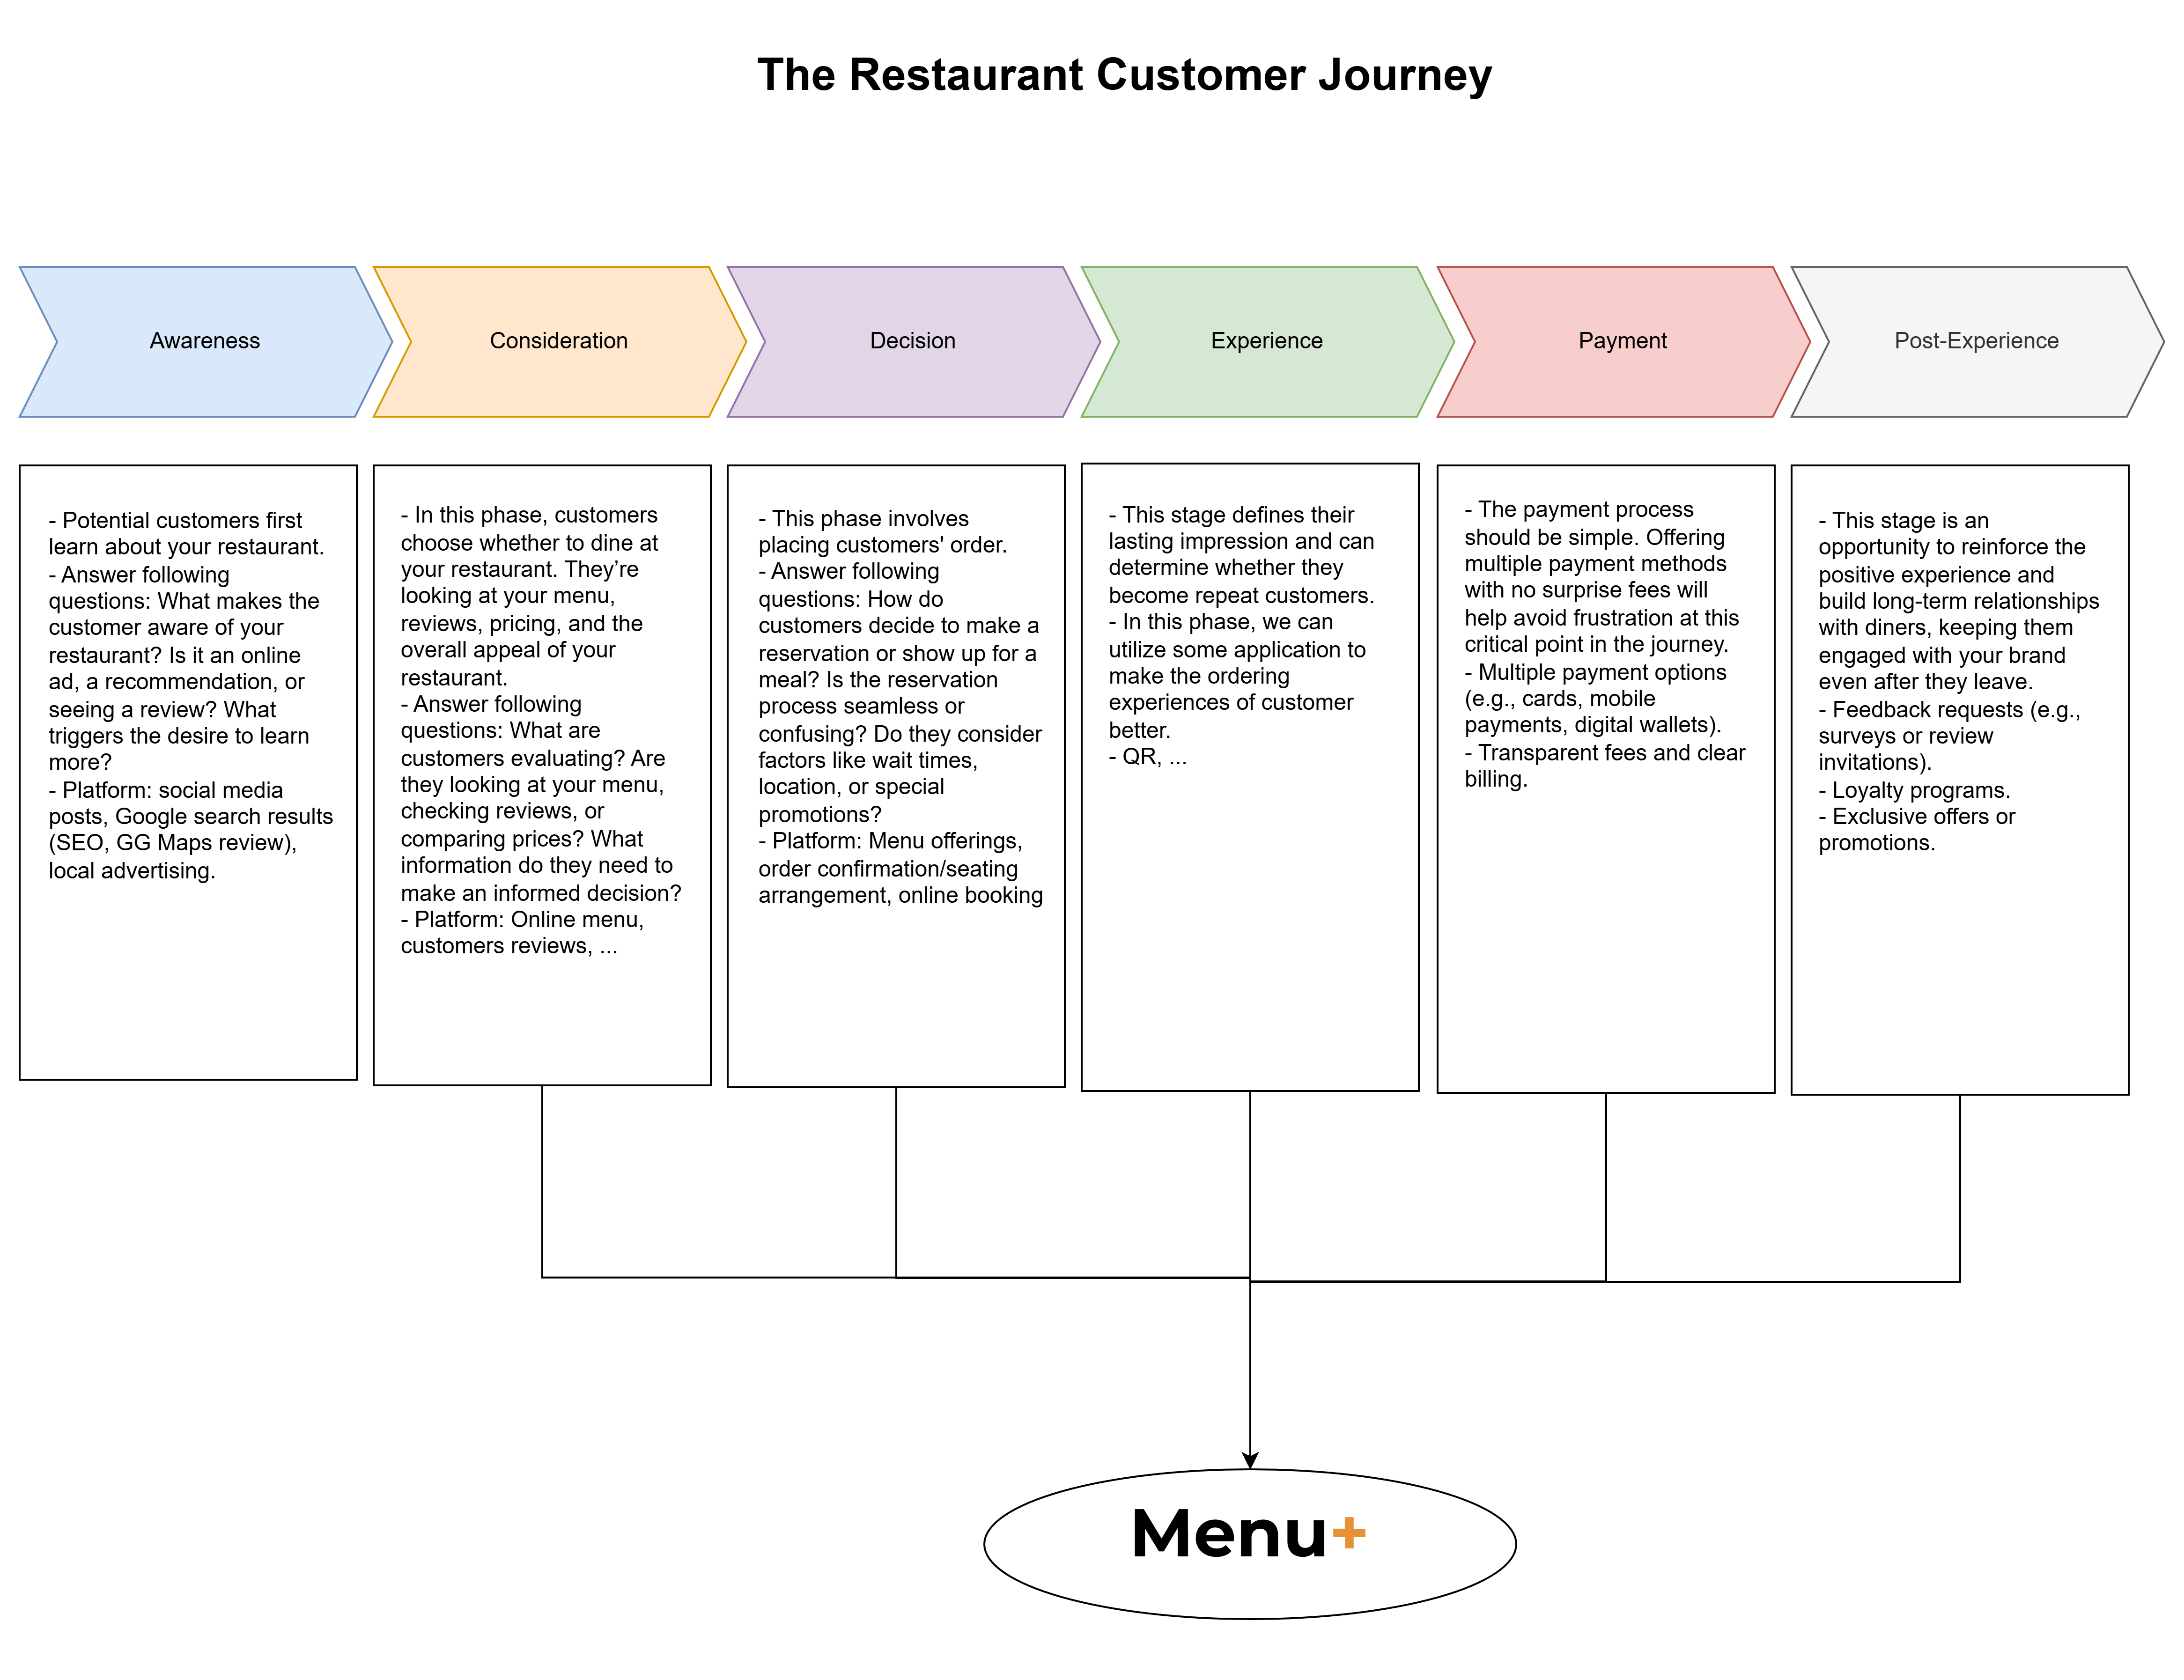
\includegraphics[width=15cm]{Images/restaurant-customer-journey.png}
%     \vspace{0.5cm}
%     \caption{Giới thiệu về Restaunrant Customer Journey}
%     \label{fig:my_label}
% \end{figure}

% % \subsubsection{Lí do chọn mục tiêu "Tích hợp và tối ưu hóa hành trình khách hàng trong dịch vụ nhà hàng"}

% Trong bối cảnh ngành dịch vụ nhà hàng ngày càng cạnh tranh khốc liệt, việc tối ưu hóa hành trình khách hàng không chỉ dừng lại ở việc nâng cao trải nghiệm mà còn trở thành một chiến lược then chốt để cải thiện hiệu quả vận hành và gia tăng lợi thế cạnh tranh. Hệ thống này tập trung vào việc tối ưu hóa các giai đoạn quan trọng trong hành trình khách hàng, bao gồm Cân nhắc, Quyết định, Trải nghiệm, Thanh toán và Hậu trải nghiệm, nhằm mang đến một quy trình đặt món, phục vụ và thanh toán liền mạch, nhanh chóng và thuận tiện. Bên cạnh đó, nhóm cũng hướng đến những mục tiêu song song quan trọng khác, bao gồm:

% \textbf{Đối với Khách hàng:}
% \begin{itemize}
%     \item \textit{Tối ưu trải nghiệm người dùng:}  Cung cấp một giao diện trực quan, thân thiện và dễ sử dụng, cho phép khách hàng dễ dàng khám phá thực đơn, thực hiện đặt món và thanh toán một cách nhanh chóng.
%     \item \textit{Tối ưu hóa trải nghiệm trong các mốc hành tình người dùng:}  Tích hợp các tính năng tiện lợi như quét mã QR để truy cập thực đơn số, đặt món theo thời gian thực và lựa chọn thanh toán linh hoạt, mang đến trải nghiệm nhất quán và không gián đoạn.
%     \item \textit{Minh bạch và tin cậy:}  Đảm bảo tính minh bạch tuyệt đối và rõ ràng trong mọi thông tin, bao gồm giá cả, các chương trình ưu đãi đặc biệt và lịch sử đặt món chi tiết.
% \end{itemize}

% \textbf{Đối với Nhân viên Nhà hàng:}
% \begin{itemize}
%     \item \textit{Nâng cao hiệu suất và độ chính xác:}  Hỗ trợ nhân viên trong việc theo dõi và xử lý các đơn hàng một cách nhanh chóng, chính xác, giảm thiểu sai sót và tăng năng suất.
%     \item \textit{Giảm tải công việc thủ công:}  Tích hợp các công cụ quản lý thông minh để giảm bớt gánh nặng công việc thủ công, từ đó giải phóng thời gian và nguồn lực cho các hoạt động quan trọng khác.
% \end{itemize}

% \textbf{Đối với Nhà Quản lý:}
% \begin{itemize}
%     \item \textit{Cung cấp công cụ hỗ trợ báo cáo và phân tích chi tiết:}  Giúp quản lý dễ dàng theo dõi doanh thu, phân tích xu hướng bán hàng và đánh giá hiệu quả hoạt động tổng thể của nhà hàng.
%     \item \textit{Quản lý hiệu quả nguồn lực:}  Tích hợp chức năng quản lý kho nguyên liệu và nhân sự, hỗ trợ việc ra quyết định nhanh chóng và hiệu quả, tối ưu hóa chi phí và đảm bảo nguồn cung ổn định.
%     \item \textit{Tính linh hoạt cao:}  Đảm bảo khả năng mở rộng và tích hợp dễ dàng các tính năng mới trong tương lai, phù hợp với sự phát triển không ngừng của nhà hàng và sự thay đổi của nhu cầu thị trường.
% \end{itemize}

% \textbf{Về mặt kỹ thuật:}

% \begin{itemize}
%     \item \textit{Hiệu suất và bảo mật tối ưu:}  Thiết kế một hệ thống có hiệu suất cao, khả năng xử lý đồng thời nhiều tác vụ và đảm bảo bảo mật tuyệt đối cho dữ liệu người dùng.
%     \item \textit{Kiến trúc linh hoạt và dễ bảo trì:}  Xây dựng một kiến trúc hệ thống linh hoạt, dễ dàng bảo trì, nâng cấp và mở rộng để đáp ứng nhu cầu phát triển trong tương lai.
% \end{itemize}


% \subsection{Mục tiêu đề tài}

% Mục tiêu của đề tài là xây dựng một hệ thống quản lý đặt món hiện đại, tích hợp các giải pháp công nghệ để tối ưu hóa quy trình vận hành nhà hàng và nâng cao trải nghiệm khách hàng, đồng thời khắc phục các hạn chế của phương pháp quản lý truyền thống đã nêu. Hệ thống này tập trung vào việc tự động hóa các quy trình từ đặt món, quản lý đơn hàng đến thanh toán, đồng thời cung cấp các công cụ phân tích và quản lý hiệu quả cho nhà hàng. Dự án hướng đến việc mang lại lợi ích thiết thực cho khách hàng, nhân viên và quản lý, góp phần thúc đẩy sự phát triển bền vững của ngành công nghiệp nhà hàng trong kỷ nguyên số.

% \begin{enumerate}
%     \item \textbf{Đối với Khách hàng:}
%         \begin{itemize}
%             \item \textit{Tối ưu trải nghiệm người dùng:} Cung cấp giao diện thân thiện, trực quan, cho phép khách hàng dễ dàng truy cập thực đơn, đặt món nhanh chóng và thanh toán linh hoạt qua các phương thức điện tử, như ví điện tử hoặc mã QR, nhằm mang lại trải nghiệm liền mạch.
%             \item \textit{Minh bạch và tin cậy:} Đảm bảo thông tin về giá cả, chương trình ưu đãi và lịch sử đặt món được trình bày rõ ràng, minh bạch, xây dựng niềm tin và sự hài lòng của khách hàng.
%             \item \textit{Cá nhân hóa trải nghiệm:} Sử dụng dữ liệu lịch sử đặt món để cung cấp các ưu đãi và khuyến mãi phù hợp, khuyến khích khách hàng quay lại và tham gia các chương trình khách hàng thân thiết.
%         \end{itemize}

%     \item \textbf{Đối với Nhân viên Nhà hàng:}
%         \begin{itemize}
%             \item \textit{Nâng cao hiệu suất và độ chính xác:} Hỗ trợ nhân viên xử lý đơn hàng nhanh chóng, giảm thiểu sai sót trong quá trình phục vụ, đặc biệt vào giờ cao điểm, thông qua các tính năng tự động hóa.
%             \item \textit{Giảm tải công việc thủ công:} Tích hợp công cụ quản lý thông minh để giảm bớt các tác vụ ghi chép thủ công, giúp nhân viên tập trung vào việc nâng cao chất lượng dịch vụ.
%         \end{itemize}

%     \item \textbf{Đối với Nhà Quản lý:}
%         \begin{itemize}
%             \item \textit{Cung cấp công cụ phân tích và báo cáo:} Hỗ trợ quản lý theo dõi doanh thu, phân tích xu hướng bán hàng và đánh giá hiệu quả hoạt động thông qua các báo cáo chi tiết, từ đó đưa ra quyết định kinh doanh chiến lược.
%             \item \textit{Quản lý hiệu quả nguồn lực:} Tích hợp chức năng quản lý kho, tối ưu hóa lịch làm việc của nhân viên và đảm bảo nguồn cung ổn định, giúp giảm chi phí và nâng cao hiệu quả vận hành.
%         \end{itemize}
% \end{enumerate}

\subsection{Mục tiêu đề tài}

Đề tài hướng đến xây dựng một \textbf{Hệ thống Quản lý Đặt món Hiện đại, Tích hợp và Hiệu quả}, đáp ứng nhu cầu vận hành của nhà hàng trong bối cảnh chuyển đổi số mạnh mẽ của ngành dịch vụ ăn uống. Hệ thống được thiết kế để vượt qua các hạn chế của phương pháp quản lý thủ công, như sai sót trong xử lý đơn hàng, giao tiếp không hiệu quả giữa các bộ phận và trải nghiệm khách hàng chưa tối ưu. Thông qua việc cung cấp giao diện thân thiện, hệ thống cho phép khách hàng dễ dàng xem thực đơn, đặt món, tùy chỉnh yêu cầu, theo dõi trạng thái đơn hàng và thanh toán nhanh chóng bằng nhiều phương thức, từ đó nâng cao sự tiện lợi và hài lòng. Đồng thời, hệ thống tối ưu hóa quy trình làm việc của nhân viên phục vụ, bếp/bar và thu ngân bằng các công cụ quản lý thông minh, giúp giảm thiểu sai sót, tăng tốc độ phục vụ và cung cấp báo cáo doanh thu chi tiết để hỗ trợ quản lý. Qua đó, hệ thống không chỉ hiện đại hóa quy trình vận hành mà còn góp phần giảm chi phí dài hạn, nâng cao hiệu quả quản lý và tạo lợi thế cạnh tranh bền vững cho nhà hàng.

% Trên cơ sở phân tích bối cảnh, động lực và những thách thức đã nêu, đề tài này đặt ra mục tiêu xây dựng một \textbf{Hệ thống Quản lý Đặt món Hiện đại, Tích hợp và Hiệu quả} cho nhà hàng. Hệ thống không chỉ nhằm giải quyết các hạn chế của phương pháp quản lý truyền thống mà còn được thiết kế để \textbf{trực tiếp đối phó và vượt qua các thách thức} đã được xác định, đáp ứng các kỳ vọng ngày càng cao của khách hàng và yêu cầu vận hành trong kỷ nguyên số.

% Các mục tiêu cụ thể của hệ thống, tập trung vào các tính năng chính và cách chúng giải quyết thách thức, bao gồm:

% \begin{enumerate}
%     \item \textbf{Đối với Khách hàng:} Nâng cao trải nghiệm đặt món và thanh toán, mang lại sự tiện lợi và chủ động.
%         \begin{itemize}
%             \item \textit{Xem thực đơn điện tử:} Truy cập thực đơn trực quan (hình ảnh, mô tả, giá cả) dễ dàng qua thiết bị di động hoặc kiosk tại bàn.
%             \item \textit{Đặt món và tùy chỉnh:} Chọn món, điều chỉnh số lượng, và dễ dàng thêm các yêu cầu đặc biệt (ví dụ: ít cay, không hành, thêm phô mai).
%             \item \textit{Theo dõi trạng thái đơn hàng:} Có thể xem được trạng thái đơn hàng của mình (đang chờ xác nhận, đang chuẩn bị, đã sẵn sàng - tùy mức độ triển khai).
%             \item \textit{Yêu cầu thanh toán và thanh toán tiện lợi:} Gọi thanh toán và thực hiện thanh toán nhanh chóng qua các phương thức đa dạng như tiền mặt, thẻ, và đặc biệt là quét mã QR ngay tại bàn (\textit{giải quyết phần nào thách thức về tích hợp thanh toán điện tử}).
%             \item \textit{Gọi phục vụ:} Có chức năng gọi nhân viên hỗ trợ khi cần thiết thông qua hệ thống.
%         \end{itemize}

%     \item \textbf{Đối với Nhân viên Phục vụ:} Tối ưu hóa quy trình nhận và chuyển đơn hàng, giảm sai sót và tăng tốc độ phục vụ.
%         \begin{itemize}
%             \item \textit{Ghi nhận đơn hàng di động:} Sử dụng máy tính bảng hoặc thiết bị POS di động để nhận đơn ngay tại bàn, giảm thiểu việc ghi chép thủ công.
%             \item \textit{Gửi đơn hàng tự động:} Đơn hàng được gửi tức thì và chính xác đến bộ phận bếp và/hoặc bar thông qua màn hình hiển thị.
%             \item \textit{Quản lý trạng thái bàn:} Dễ dàng theo dõi trạng thái các bàn (trống, đang có khách, đã đặt trước, cần dọn dẹp).
%             \item \textit{Xử lý yêu cầu đặc biệt:} Ghi chú và chuyển các yêu cầu đặc biệt của khách hàng một cách rõ ràng.
%             \item \textit{Hỗ trợ thanh toán tại bàn:} Thực hiện quy trình thanh toán (in hóa đơn tạm, xác nhận thanh toán) hiệu quả hơn.
%         \end{itemize}

%     \item \textbf{Đối với Nhân viên Bếp/Bar:} Nhận thông tin đơn hàng chính xác và kịp thời, tối ưu hóa quy trình chế biến.
%         \begin{itemize}
%             \item \textit{Hiển thị đơn hàng điện tử (Kitchen Display System - KDS):} Nhận đơn hàng rõ ràng trên màn hình, bao gồm chi tiết món và các tùy chỉnh, thay vì phiếu giấy dễ thất lạc hoặc nhòe mực.
%             \item \textit{Quản lý thứ tự chế biến:} Hệ thống có thể hỗ trợ sắp xếp thứ tự ưu tiên của các đơn hàng hoặc món ăn.
%             \item \textit{Đánh dấu trạng thái món ăn:} Thông báo cho bộ phận phục vụ khi món ăn đã sẵn sàng để phục vụ.
%         \end{itemize}

%     \item \textbf{Đối với Nhân viên Thu ngân và Quản lý:} Cung cấp công cụ quản lý hiệu quả, theo dõi doanh thu và hiệu suất hoạt động.
%         \begin{itemize}
%             \item \textit{Quản lý hóa đơn và thanh toán tập trung:} Dễ dàng xem lại, in ấn, và xử lý thanh toán cho các hóa đơn.
%             \item \textit{Áp dụng khuyến mãi, giảm giá:} Hệ thống hỗ trợ việc thiết lập và áp dụng các chương trình khuyến mãi một cách linh hoạt.
%             \item \textit{Báo cáo doanh thu chi tiết:} Cung cấp các báo cáo doanh thu theo thời gian (ngày, tuần, tháng), theo món ăn, theo nhân viên, giúp quản lý nắm bắt tình hình kinh doanh.
%             \item \textit{Quản lý thực đơn và giá bán:} Cho phép quản lý dễ dàng cập nhật thực đơn, giá cả và mô tả món ăn.
%             \item \textit{Quản lý tài khoản người dùng:} Phân quyền truy cập và sử dụng hệ thống cho từng vai trò nhân viên.
%         \end{itemize}

%     \item \textbf{Mục tiêu Hệ thống Tổng thể - Trực tiếp giải quyết các thách thức cốt lõi:}
%         \begin{itemize}
%             \item \textit{Tính ổn định và hiệu năng:} Đảm bảo hệ thống hoạt động mượt mà, ổn định, đặc biệt trong các giờ cao điểm, giảm thiểu tối đa thời gian chết (\textit{giải quyết thách thức về quản lý lỗi và vận hành liên tục}).
%             \item \textit{Tính bảo mật cao:} Xây dựng các cơ chế bảo mật mạnh mẽ để bảo vệ dữ liệu giao dịch, thông tin khách hàng và dữ liệu kinh doanh, tuân thủ các quy định pháp luật (\textit{giải quyết thách thức về bảo mật dữ liệu và quyền riêng tư}).
%             \item \textit{Kiến trúc linh hoạt và khả năng tích hợp:} Thiết kế hệ thống theo kiến trúc module, sử dụng các API rõ ràng để dễ dàng tích hợp với các thiết bị phần cứng phổ biến (máy in, máy POS) và có thể mở rộng để tích hợp với các hệ thống khác (kế toán, kho) trong tương lai (\textit{giải quyết thách thức về độ phức tạp kỹ thuật và tích hợp hệ thống}).
%             \item \textit{Giao diện thân thiện và trực quan (UX/UI):} Ưu tiên thiết kế giao diện người dùng đơn giản, dễ học, dễ sử dụng cho tất cả các đối tượng, từ khách hàng đến nhân viên và quản lý, nhằm giảm thời gian đào tạo và tăng tỷ lệ chấp nhận (\textit{giải quyết thách thức về thiết kế trải nghiệm người dùng và đào tạo/thay đổi thói quen}).
%             \item \textit{Quản lý dữ liệu hiệu quả:} Thiết kế cơ sở dữ liệu tối ưu để xử lý khối lượng lớn giao dịch và thông tin, đảm bảo khả năng truy vấn và báo cáo nhanh chóng (\textit{giải quyết thách thức về quản lý dữ liệu lớn}).
%             % Lưu ý: Thách thức về chi phí, thời gian và nhân lực được giải quyết thông qua việc lập kế hoạch dự án, lựa chọn công nghệ phù hợp và quản lý hiệu quả, hơn là một tính năng trực tiếp của hệ thống. Tuy nhiên, một hệ thống hiệu quả, dễ sử dụng và bảo trì sẽ góp phần giảm chi phí vận hành và đào tạo dài hạn.
%         \end{itemize}
% \end{enumerate}

% Việc đạt được các mục tiêu này không chỉ mang lại các tính năng mong đợi mà còn trực tiếp tháo gỡ những rào cản và khó khăn đã được nhận diện. Qua đó, hệ thống sẽ góp phần hiện đại hóa quy trình vận hành, nâng cao sự hài lòng của khách hàng, tăng cường hiệu quả quản lý và tạo lợi thế cạnh tranh bền vững cho nhà hàng trong bối cảnh ngành F\&B đang chuyển đổi số mạnh mẽ.
